\documentclass[t,hyperref={bookmarks=false}]{beamer}

\usepackage{lmodern}
\usepackage[utf8]{inputenc}
\usepackage[T1]{fontenc}
\usepackage{microtype}
\usepackage[english,shorthands=off]{babel}
\usepackage{mathtools}
\usepackage{mathabx}
\usepackage{dsfont}
\usepackage{mathdots}
\usepackage{comment}
\usepackage{graphicx}

\usepackage{tensor}
\newcommand{\ind}{\indices}
\newcommand{\pd}{\partial}

%Tikz
\usepackage{tikz}
%Tikz-cd - Commutative diagrams (Tikz)
\usetikzlibrary{cd}
\usetikzlibrary{shapes.multipart}
\usetikzlibrary{shadings}
\tikzset{%document wide settings
  %append settings to 'every label':
  /tikz/commutative diagrams/labels={font=\normalsize},
  %append options to the style 'every arrow'
  /tikz/commutative diagrams/arrows={-stealth},
  /tikz/ampersand replacement=\&,
  /tikz/commutative diagrams/background color=white!90!black
}

\mode<presentation>
{
  \usetheme{Malmoe}
  \usecolortheme{spruce}
  \usecolortheme{rose}
  \useoutertheme{hendrik}
  \setbeamercovered{transparent}

  \setbeamercolor{section in toc}{fg=blue!65!yellow!80!black}
  \setbeamertemplate{blocks}[rounded]
  \setbeamercolor{alerted text}{fg=black!20!red}
  \setbeamercolor{block title}{%
    fg=MSUgreen!60!black, bg=white!90!black}
  \setbeamercolor{block body}{bg=white!90!black}
  \setbeamertemplate{itemize item}[square]
  \setbeamertemplate{itemize subitem}{$\bullet$}
  \setbeamercolor{itemize item}{fg=blue!65!yellow!95!black}
  \setbeamercolor{itemize 
    subitem}{fg=blue!65!yellow!80!red!90!white}
}

\beamertemplatenavigationsymbolsempty

\newcommand{\bitem}{\begin{itemize}}
\newcommand{\eitem}{\end{itemize}}
\newcommand{\mrm}{\mathrm}
\usepackage{scalerel}
\newcommand{\dal}{\raisebox{-1.73pt}{%
    \scaleobj{2.07}{\square}\hspace{-0.1111em}}}

\title{Dark energy as a kinematic effect}
\subtitle{Merging de Sitter special relativity with teleparallel 
  gravity}
\author[Hendrik Jennen]{%
  Hendrik Jennen\texorpdfstring{\\
    \vspace{\baselineskip}
  \footnotesize{Supervisor: José Geraldo Pereira}
  }{}
}
\institute{Instituto de Física Teórica - UNESP
  \vspace{2\baselineskip}}
\date{\footnotesize{February 12, 2016}}

\begin{document}

\frame{\titlepage}
\begin{frame}{Outline}
  \tableofcontents
\end{frame}

\section{Motivation}

\subsection{Accelerated expansion \& de Sitter kinematics}

\begin{frame}{Cosmological principle}

\bitem
  \item<1-> Homogeneous and isotropic universe at large scales
    \bitem
      \item $\sim 300$ million light-years
    \eitem
\eitem

\visible<2->{
\begin{block}<2->{Friedman-Lemaître-Robertson-Walker}
  \begin{equation*}
    ds^2 = dt^2 - \alert<4>{a(t)}^2 \big[ d\chi^2
    + \alert<3>{f_{k}(\chi)}^2\, d\Omega_2 \big]
  \end{equation*}
\end{block}

\bitem
  \item<2-> Comoving coordinates
  \item<2-> Symmetric universe / cosmological principle
  \item<3-> Space with constant curvature
    \bitem
      \item \makebox[4cm][l]{Spherical for $k = 1$} $[f_k = \sin 
        \chi]$
      \item \makebox[4cm][l]{Flat for $k = 0$} [$f_k = \chi$]
      \item \makebox[4cm][l]{Hyperbolic for $k = -1$} [$f_k 
        = \sinh\chi$]
      \eitem
  \item<4-> Scale factor
\eitem
}
\end{frame}

\begin{frame}{Present-day accelerated expansion}

\bitem
  \item<1-> Determine evolution of scale factor today $(t_*)$
    \bitem
      \item No a-priori assumptions on dynamical model
    \eitem
  \item<1-> Luminosity distance $d_L$ vs.~redshift $z$ for SNe Ia
    \bitem
      \item $d_L^2 \sim L_\text{absolute}/F_\text{observed}$
      \item $z = a_*/a - 1$
    \eitem
\eitem

\visible<2->{%
\begin{block}<2->{Hubble law}
  \vspace{-\baselineskip}
  \begin{equation*}
    d_L(z) = \frac{z}{H_*} + [1-q_*]\frac{z^2}{2H_*}
    - \Big[1 - q_* -3q_*^2 + j_* + \alert<3>{\frac{k}{a_*^2 
        H_*^2}} \Big] \frac{z^3}{6H_*} \end{equation*}
\end{block}

\bitem
  \item<2-> $H = \dot{a}/a$,\quad $q = -\ddot{a}a/\dot{a}^2$,
    \quad $j = \dddot{a}a^2/\dot{a}^3$, \quad\ldots
  \item<3-> Inflation $\implies$ negligible curvature term
  \item<4-> Evidence for accelerated
    expansion~~$\longleftrightarrow$~~$\dot{a}_*, \ddot{a}_* > 0$
\eitem
}
\end{frame}

\begin{frame}{Dark energy}

\begin{block}{Einstein's equations}
  \begin{equation*}
    R\ind{_{\mu\nu}} - g\ind{_{\mu\nu}} R
    \uncover<2->{+ g\ind{_{\mu\nu}} \alert<2>{\Lambda}}
    = T\ind{_{\mu\nu}}
  \end{equation*}
  \vspace{-\baselineskip}
\end{block}

\bitem
\item No known component of repulsive gravitation
\item Expansion driven by dark energy
\item<2-> Cosmological constant
\item<2-> Vacuum solution given by de Sitter space
\eitem
\bitem
\item<3-> Change of large-scale kinematic group
  \bitem
    \item $ISO(1,3) \longrightarrow SO(1,4)$
    \item Degree of deformation depends on $\Lambda$
    \item de Sitter special relativity
  \eitem
\eitem

\end{frame}

\begin{frame}{Cosmological function}

\begin{block}{Working objective}
  \centering
  Kinematic group at every point is $SO(1,4)$
\end{block}

\bitem
  \item Pointwise deformation $ISO(1,3) 
    \overset{\Lambda}{\longrightarrow} SO(1,4)$
    \bitem
      \item How much varies from event to event
    \eitem
  \item $\Lambda$ becomes nonconstant function
    \bitem
      \item Cosmological function
    \eitem
\eitem
\vspace{0.8\baselineskip}
\visible<2->{%
\bitem
  \item How to implement mathematically?
    \bitem
      \item Cartan geometry modeled on de Sitter space
    \eitem
  \item How to implement physically?
    \bitem
      \item Generalize teleparallel gravity
      \item Deform curvature of spin connection
    \eitem
\eitem
}
\end{frame}

\section{Cartan geometry}

\subsection{Geometry of spacetime}

\begin{frame}{Klein geometry}

\visible<2->{
\bitem
\item Geometry of homogeneous spaces
  \bitem
  \item Minkowski space, de Sitter space, $\ldots$
  \eitem
\item Symmetry Lie group $G$ $\longrightarrow$ transitivity
  \bitem
  \item $ISO(1,3)$, $SO(1,4)$, $\ldots$
  \eitem
\item Subgroup $H \subset G$ defines isotropy around any point
  \bitem
  \item $SO(1,3)$, $SO(1,3)$, $\ldots$
  \eitem
\item Homogeneous space $\longleftrightarrow$ $G/H$
\eitem
}

\visible<3->{
\begin{center}
\begin{tikzpicture}[
  cellH/.style={%
    rectangle split,
    rectangle split horizontal,
    rectangle split parts=2,
    rectangle split part fill={white!90!black,
      MSUgreen!20!white},
    rounded corners,
    font=\footnotesize
  },
  cellV/.style={%
    rectangle split,
    rectangle split parts=2,
    rounded corners,
    rectangle split part fill={white!90!black,
      MSUgreen!20!white},
    font=\footnotesize
  },
  line/.style={%
    draw,
    semithick,
    -stealth,
    shorten >=5pt, shorten <=5pt
  }
]
\matrix [column sep=1.8cm, row sep=1.3cm]
{%
\node [cellH] (mink)
  {Minkowski space\nodepart{two}%
    $ISO(1,3)$}; \&
\node [cellH] (desit)
  {de Sitter space \nodepart{two}%
    $SO(1,4)$}; \\
\visible<4->{%
\node [cellV] (riem)
  {Riemann--Cartan space\nodepart{two}%
    local $ISO(1,3)$};} \&
\visible<5->{%
\node [cellV] (cartan)
  {Cartan geometry\nodepart{two}%
    local $SO(1,4)$};} \\
};
\path [line] (mink) --
      node [above,font=\footnotesize] {$\Lambda$} (desit);
\visible<4->{%
\path [line] (mink) --
      node [right,font=\footnotesize] {gravity} (riem);}
\visible<5->{%
\path [line] (riem) --
      node [above,font=\footnotesize] {$\Lambda$}
      node [below,font=\footnotesize] {$d\Lambda \neq 0$} 
      (cartan);
\path [line] (desit) --
      node [right,font=\footnotesize] {gravity} (cartan);}
\end{tikzpicture}
\end{center}
}

\end{frame}

\begin{frame}{Cartan geometry}

\bitem
\item Let $G/H$ be homogeneous model space
\item Give up homogeneity, retain symmetry locally
\item<2-> Endow manifold $M$ with Cartan connection $A$
  \bitem
  \item 1-form valued in $\mathfrak{g}$
  \item $\dim M = \dim G/H$
  \eitem
\eitem

\begin{block}<2->{Cartan connection}
  \begin{equation*}
  A: TM \mapsto \mathfrak{g} = \mathfrak{h} \oplus 
  \mathfrak{g}/\mathfrak{h}
\end{equation*}
\end{block}

\visible<3->{
\begin{columns}[c]
\column[c]{0.3\textwidth}
  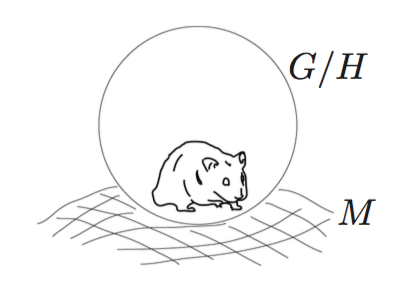
\includegraphics[height=2.7cm]{hamster.png}
\column{0.6\textwidth}
  \bitem
  \item $G = SO(3)$, $H = SO(2)$
  \item For each direction, $A$ returns\\
    an element of $\mathfrak{so}(3)$
  \eitem
\end{columns}
}

\end{frame}

\begin{frame}{Cartan geometry}
\begin{block}{Cartan connection}
  \begin{equation*}
  A: TM \mapsto \mathfrak{g} = \mathfrak{h} \oplus 
  \mathfrak{g}/\mathfrak{h}
\end{equation*}
\end{block}

\bitem
\item $A_\mathfrak{h}$ is $H$-connection
\item $A_\mathfrak{p}$ is vielbein $\longrightarrow$ soldering
\eitem

\begin{block}<2->{Cartan curvature}
  \begin{equation*}
    F = dA + \frac{1}{2}[A,A]
  \end{equation*}
\end{block}

\bitem
\item<2-> $F_\mathfrak{h}$ is curvature
\item<2-> $F_\mathfrak{p}$ is torsion
\item<2-> $F = 0 \iff M = G/H$
\eitem
\end{frame}

\subsection{de Sitter--Cartan geometry}

\begin{frame}{de Sitter space \& Lie algebra}

\bitem
\item Generic spacetime with locally $SO(1,4)$ kinematics
\item Homogeneous model space: $SO(1,4)/SO(1,3)$
\eitem

\visible<2->{
\begin{block}{de Sitter algebra}
  \begin{equation*}
    \mathfrak{so}(1,4) = \mathfrak{so}(1,3) \oplus 
    \mathfrak{p}
  \end{equation*}
\end{block}

\bitem
\item de Sitter translations \hspace{0.3cm} $[\mathfrak{p} 
  = \mathfrak{so}(1,4) / \mathfrak{so}(1,3)]$
\only<4->{%
\item<4-> Splitting is $SO(1,3)$ invariant
\item<5-> Length scale hidden in translations
  \bitem
  \item Cosmological constant
  \item $\Lambda \to 0$ gives Minkowski space
  \item $\mathfrak{p}$ $\longrightarrow$ Poincar\'e translations
  \eitem
}
}
\eitem

\only<2,3>{
\begin{block}{Commutation relations}
  \vspace{-0.8\baselineskip}
  \begin{align*}
    [\mathfrak{so}(1,3), \mathfrak{so}(1,3)] &\subset 
    \mathfrak{so}(1,3) \\
    \alert<3>{[\mathfrak{so}(1,3), \mathfrak{p}]}
    &\alert<3>{\subset \mathfrak{p}} \\
    [\mathfrak{p}, \mathfrak{p}] &\subset \mathfrak{so}(1,3)
  \end{align*}
\end{block}}

\end{frame}

\begin{frame}{de Sitter--Cartan geometry}

\bitem
\item Provide spacetime with de Sitter--Cartan connection
\item At every point valued in copies of $\mathfrak{so}(1,4)$
  \bitem
  \item Let length scale in $\mathfrak{p}$ vary pointwise
  \eitem
\item Cosmological function $\Lambda$
\eitem

\only<2->{
\vspace{-10pt}
\begin{columns}[t,onlytextwidth]
\column{0.48\textwidth}
\begin{block}{\centering{Spin connection \& vierbein}}
\vspace{-0.854\baselineskip}
\begin{equation*}
  \begin{tikzcd}[column sep=2.2cm, row sep=-5pt, 
    labels={font=\footnotesize}]
      {}  \& \omega\ind{^a_{b\mu}} \\
      A   \arrow[ru, "{\mathfrak{so}(1,3)}" description,
                  rounded corners,
                  curve to, out=40, in=180, looseness=0.5,
                  start anchor={[xshift=-2pt, yshift=-2pt]north 
                    east},
                  end anchor=west]
          \arrow[rd, "{\mathfrak{p}}" description,
                  rounded corners,
                  curve to, out=-40, in=180, looseness=0.4,
                  start anchor={[xshift=-2pt, yshift=+2pt]south 
                    east},
                  end anchor={[xshift=-2.5pt]west}]
            \& \\
          \& e\ind{^a_\mu}
  \end{tikzcd}%
\end{equation*}
\end{block}

\column{0.48\textwidth}
\begin{block}{\centering{Curvature \& torsion}}
\vspace{-0.8\baselineskip}
\begin{equation*}
  \begin{tikzcd}[column sep=2.2cm, row sep=-5pt, 
    labels={font=\footnotesize}]
      {}  \& R\ind{^a_{b\mu\nu}} \\
      F   \arrow[ru, "{\mathfrak{so}(1,3)}" description,
                  rounded corners,
                  curve to, out=40, in=180, looseness=0.5,
                  start anchor={[xshift=-2pt, yshift=-2pt]north 
                    east},
                  end anchor=west]
          \arrow[rd, "{\mathfrak{p}}" description,
                  rounded corners,
                  curve to, out=-40, in=180, looseness=0.4,
                  start anchor={[xshift=-2pt, yshift=+2pt]south 
                    east},
                  end anchor={[xshift=-2pt]west}]
            \& \\
          \& T\ind{^a_{\mu\nu}}
  \end{tikzcd}%
\end{equation*}
\end{block}
\end{columns}

\bitem
\item Decompose according to $\mathfrak{so}(1,4) 
  = \mathfrak{so}(1,3) \oplus \mathfrak{p}$
\item Local $SO(1,3)$ invariance
\item $F = dA + \tfrac{1}{2}[A,A]$
\eitem
}

\end{frame}

\begin{frame}{de Sitter--Cartan geometry}

\vspace{-20pt}
\begin{columns}[t,onlytextwidth]
\column{0.48\textwidth}
\begin{block}{\centering{Spin connection \& vierbein}}
\vspace{-0.854\baselineskip}
\begin{equation*}
  \begin{tikzcd}[column sep=2.2cm, row sep=-5pt, 
    labels={font=\footnotesize}]
      {}  \& \omega\ind{^a_{b\mu}} \\
      A   \arrow[ru, "{\mathfrak{so}(1,3)}" description,
                  rounded corners,
                  curve to, out=40, in=180, looseness=0.5,
                  start anchor={[xshift=-2pt, yshift=-2pt]north 
                    east},
                  end anchor=west]
          \arrow[rd, "{\mathfrak{p}}" description,
                  rounded corners,
                  curve to, out=-40, in=180, looseness=0.4,
                  start anchor={[xshift=-2pt, yshift=+2pt]south 
                    east},
                  end anchor={[xshift=-2.5pt]west}]
            \& \\
          \& e\ind{^a_\mu}
  \end{tikzcd}%
\end{equation*}
\end{block}

\column{0.48\textwidth}
\begin{block}{\centering{Curvature \& torsion}}
\vspace{-0.8\baselineskip}
\begin{equation*}
  \begin{tikzcd}[column sep=2.2cm, row sep=-5pt, 
    labels={font=\footnotesize}]
      {}  \& R\ind{^a_{b\mu\nu}} \\
      F   \arrow[ru, "{\mathfrak{so}(1,3)}" description,
                  rounded corners,
                  curve to, out=40, in=180, looseness=0.5,
                  start anchor={[xshift=-2pt, yshift=-2pt]north 
                    east},
                  end anchor=west]
          \arrow[rd, "{\mathfrak{p}}" description,
                  rounded corners,
                  curve to, out=-40, in=180, looseness=0.4,
                  start anchor={[xshift=-2pt, yshift=+2pt]south 
                    east},
                  end anchor={[xshift=-2pt]west}]
            \& \\
          \& T\ind{^a_{\mu\nu}}
  \end{tikzcd}%
\end{equation*}
\end{block}
\end{columns}

\begin{block}{}
\vspace{-\baselineskip}
\begin{align*}
  R\ind{^a_{b\mu\nu}} &= B\ind{^a_{b\mu\nu}} + \frac{\Lambda}{3} 
  (e\ind{^a_\mu} e\ind{_{b\nu}} - e\ind{^a_\nu} e\ind{_{b\mu}})
  \\
  T\ind{^a_{\mu\nu}} &= G\ind{^a_{\mu\nu}} + \frac{1}{2} \pd_\mu 
  \! \ln \Lambda\, e\ind{^a_\nu} - \frac{1}{2} \pd_\nu \! \ln 
  \Lambda\, e\ind{^a_\mu},
\end{align*}
\end{block}

\vspace{-0.22\baselineskip}
\begin{block}{}
\vspace{-\baselineskip}
\begin{align*}
  B\ind{^a_{b\mu\nu}} &= \pd_\mu \omega\ind{^a_{b\nu}} - \pd_\nu 
  \omega\ind{^a_{b\mu}} + \omega\ind{^a_{c\mu}} 
  \omega\ind{^c_{b\nu}} - \omega\ind{^a_{c\nu}} 
  \omega\ind{^c_{b\mu}}\\
  G\ind{^a_{\mu\nu}} &= \pd_\mu e\ind{^a_\nu} - \pd_\nu 
  e\ind{^a_\mu} + \omega\ind{^a_{b\mu}} e\ind{^b_\nu} 
  - \omega\ind{^a_{b\nu}} e\ind{^b_\mu}
\end{align*}
\end{block}

\bitem
\item<2-> $\Lambda \to 0$ gives back Riemann--Cartan geometry
\eitem

\end{frame}

\section{Teleparallel gravity}

\subsection{Weitzenb\"ock geometry}

\begin{frame}{Introduction to teleparallel gravity}

\bitem
\item Description for classical gravity
\item Predictions equivalent to general relativity
\item Mathematical structure is related but different
  \bitem
  \item Riemann--Cartan spacetime without curvature
  \item Gravitational degrees of freedom encoded in torsion
  \eitem
\item Conceptually quite unlike general relativity
  \bitem
  \item No geometrization of gravitational interaction
  \item Restores the concept of force
  \item Inertial and gravitational effects separated
  \eitem
\eitem

\visible<2->{%
\vspace{0.6\baselineskip}
\bitem
\item Gauge theory for the Poincar\'e translations
  \bitem
  \item Nonlinear realization of Riemann--Cartan connection
  \item Not further considered
\eitem
\eitem
}

\end{frame}

\begin{frame}{Geometric objects}

\bitem
\item Kinematics ruled by Poincar\'e group
  \bitem
  \item Riemann--Cartan geometry
  \eitem
\eitem

\begin{block}{}
\vspace{-\baselineskip}
\begin{align*}
  B\ind{^a_{b\mu\nu}} &= \pd_\mu \omega\ind{^a_{b\nu}} - \pd_\nu 
  \omega\ind{^a_{b\mu}} + \omega\ind{^a_{c\mu}} 
  \omega\ind{^c_{b\nu}} - \omega\ind{^a_{c\nu}} 
  \omega\ind{^c_{b\mu}}\\
  G\ind{^a_{\mu\nu}} &= \pd_\mu e\ind{^a_\nu} - \pd_\nu 
  e\ind{^a_\mu} + \omega\ind{^a_{b\mu}} e\ind{^b_\nu} 
  - \omega\ind{^a_{b\nu}} e\ind{^b_\mu}
\end{align*}
\end{block}

\uncover<2->{%
\begin{columns}[c, onlytextwidth]
\column{0.48\textwidth}
\begin{block}{Ricci theorem}
  \begin{equation*}
    \omega\ind{^a_{b\mu}} = \mathring{\omega}\ind{^a_{b\mu}} 
    + K\ind{^a_{b\mu}}
  \end{equation*}
\end{block}

\column{0.48\textwidth}
\bitem
\item Levi-Civita connection
\item Contortion
\eitem
\end{columns}
}

\vspace{0.5\baselineskip}
\bitem
\item<3-> General relativity $\longrightarrow$ 
  $G\ind{^a_{\mu\nu}} \equiv 0$
  \bitem
  \item $K\ind{^a_{b\mu}} = 0$
  \item Riemannian spacetime
  \item Both inertial and gravitational effects in spin 
    connection
  \eitem
\eitem

\end{frame}

\begin{frame}{Weitzenb\"ock geometry}

\begin{block}{}
\vspace{-\baselineskip}
\begin{align*}
  B\ind{^a_{b\mu\nu}} &= \pd_\mu \omega\ind{^a_{b\nu}} - \pd_\nu 
  \omega\ind{^a_{b\mu}} + \omega\ind{^a_{c\mu}} 
  \omega\ind{^c_{b\nu}} - \omega\ind{^a_{c\nu}} 
  \omega\ind{^c_{b\mu}}\\
  G\ind{^a_{\mu\nu}} &= \pd_\mu e\ind{^a_\nu} - \pd_\nu 
  e\ind{^a_\mu} + \omega\ind{^a_{b\mu}} e\ind{^b_\nu} 
  - \omega\ind{^a_{b\nu}} e\ind{^b_\mu}
\end{align*}
\end{block}

\bitem
\item Teleparallel gravity $\longrightarrow$ $B\ind{^a_{b\mu\nu}} 
  \equiv 0$
\item $\omega\ind{^a_{b\mu}} = \Lambda\ind{^a_c} \pd_\mu 
  \Lambda\ind{_b^c}$
  \bitem
  \item Spin connection encodes inertial effects only
  \eitem
\item<2-> Torsion represents gravitational degrees of freedom
\item<2-> 10 off-shell degrees of freedom
  \bitem
  \item Same as in Riemannian spacetime
  \eitem
\item<3-> Dictionary general relativity -- teleparallel gravity
  \begin{equation*}
    \mathring{\omega}\ind{^a_{b\mu}} \longleftrightarrow 
    \omega\ind{^a_{b\mu}} - K\ind{^a_{b\mu}}
    \end{equation*}
\eitem
\end{frame}

\subsection{Equations of motion}

\begin{frame}{Particle mechanics}

\begin{columns}[c,onlytextwidth]

\column{0.45\textwidth}
\begin{block}{Action}
\vspace{-0.8\baselineskip}
  \begin{equation*}
    -m \int d\tau = -m \int u_a e^a
  \end{equation*}
\end{block}

\column{0.51\textwidth}
\bitem
\item Mass $m$ in gravitational field
\item Nonzero torsion
\eitem
\end{columns}

\begin{block}<2->{Equations of motion}
  \begin{equation*}
    u^\rho D_\rho u^a = K\ind{^a_{b\rho}} u^b u^\rho
  \end{equation*}
\end{block}

\bitem
\item<2-> Inertial vs. gravitational effects
\item<2-> Force equation
\visible<3->{%
\item Equivalence with geodesic equation
  \begin{equation*}
    u^\rho \pd_\rho u^a + [ \underbrace{\omega\ind{^a_{b\rho}} 
      - K\ind{^a_{b\rho}}}_{\displaystyle 
      \mathring{\omega}\ind{^a_{b\rho}}} ] u^b u^\rho = 0
  \end{equation*}
}
\eitem

\end{frame}

\begin{frame}{Gravitional field equations}

\begin{block}{Lagrangian teleparallel gravity}
\begin{equation*}
  \mathcal{L}_\text{tg} = \frac{1}{4} G \ind{^\rho_{\mu\nu}} 
  G\ind{_\rho^{\mu\nu}} + \frac{1}{2} G\ind{^\rho_{\mu\nu}} 
  G\ind{^{\nu\mu}_\rho} - G\ind{^\nu_{\mu\nu}} 
  G\ind{^{\rho\mu}_\rho}
\end{equation*}
\end{block}

\begin{block}<2->{Field equations}
\begin{equation*}
  D_\rho (e\, W\ind{_a^{\rho\mu}}) + e\, t\ind{_a^\mu} = 0
\end{equation*}
\end{block}

\bitem
\item<2-> Superpotential $W\ind{_a^{\rho\mu}}$
\item<2-> Gravitational energy-momentum current $t\ind{_a^\mu}$
  \bitem
  \item Conserved charges $q_a = \int t\ind{_a^0} 
    \;\longrightarrow\;\dot{q}_a = 0$
  \eitem
  \eitem\bitem
\item<3-> Equivalence with general relativity
  \bitem
  \item
    $\mathcal{L}_\text{tg} \longleftrightarrow R - \pd_\mu (e\, 
    K\ind{^{\mu\nu}_\nu})$
  \eitem
\eitem
\end{frame}

\section{de Sitter teleparallel gravity}

\subsection{Fundamentals}

\begin{frame}{Introduction to de Sitter teleparallel gravity}

\visible<2->{%
\bitem
\item Deform local kinematics $ISO(1,3) \longrightarrow SO(1,4)$
\item Riemann--Cartan spacetime $\longrightarrow$ de 
  Sitter--Cartan spacetime
\item New paradigm to incorporate cosmological function
  \bitem
  \item Applicable to any theory of gravity
  \item Merging de Sitter special relativity with gravity
  \eitem
\eitem
}

\visible<3->{%
\bitem
\item de Sitter teleparallel gravity
\item Deform the curvature of spin connection
  \bitem
  \item Minkowski space $\longrightarrow$ de Sitter space
  \item Deformation specified by $\Lambda$
  \item Kinematic contribution to deviation equation
  \eitem
\item Gravity relates to torsion of vierbein
\item Cosmological function acquires own dynamics
\eitem
}

\end{frame}

\begin{frame}{Fundamentals}

\bitem
\item Kinematics ruled by de Sitter group
  \bitem
  \item de Sitter--Cartan geometry
  \eitem
\begin{block}{}
\vspace{-\baselineskip}
\begin{align*}
  R\ind{^a_{b\mu\nu}} &= B\ind{^a_{b\mu\nu}} + \frac{\Lambda}{3} 
  (e\ind{^a_\mu} e\ind{_{b\nu}} - e\ind{^a_\nu} e\ind{_{b\mu}})
  \only<3->{\alert<3>{\equiv 0}}
  \\
  T\ind{^a_{\mu\nu}} &= G\ind{^a_{\mu\nu}} + \frac{1}{2} \pd_\mu 
  \! \ln \Lambda\, e\ind{^a_\nu} - \frac{1}{2} \pd_\nu \! \ln 
  \Lambda\, e\ind{^a_\mu},
\end{align*}
\end{block}
\eitem

\bitem
\item<2-> Gravitational field $\iff$ $G\ind{^a_{\mu\nu}} \neq 0$
\eitem

\visible<3->{%
\begin{block}{Kinematic curvature}
\begin{equation*}
    B\ind{^a_{b\mu\nu}} = - \frac{\Lambda}{3} (e\ind{^a_\mu} 
    e\ind{_{b\nu}} - e\ind{^a_\nu} e\ind{_{b\mu}})
\end{equation*}
\end{block}

\bitem
\item<4-> $\Lambda \to 0$ \hspace{0.1cm} $\longrightarrow$ 
  Weitzenb\"ock spacetime
\eitem
}

\end{frame}

\begin{frame}{Particle mechanics \& kinematic effects}

\vspace{-1.5\baselineskip}
\begin{columns}[t,onlytextwidth]
\column{0.35\textwidth}
\begin{block}{Action}
\vspace{-0.49\baselineskip}
  \begin{equation*}
    -m \int u_a e^a
  \end{equation*}
\end{block}

\column{0.61\textwidth}
\begin{block}{Equations of motion}
  \begin{equation*}
    u^\rho D_\rho u^a = K\ind{^a_{b\rho}} u^b u^\rho
  \end{equation*}
\end{block}
\end{columns}
\vspace{0.2\baselineskip}

\bitem
\item Formally the same as in teleparallel gravity
\item<2-> $\Lambda$ affects deviation free-falling particles
\eitem

\visible<3->{%
\vspace{-0.3\baselineskip}
\begin{columns}[c,onlytextwidth]

\column{0.72\textwidth}
\vspace{-0.61\baselineskip}
\bitem
\item String of free-falling particles $x_\sigma(\tau)$
  \bitem
  \item $\sigma$ runs along the string $\longrightarrow 
    v = d/d\sigma$
  \item $\tau$ is the proper time $\longrightarrow u = d/d\tau$
  \item Relative acceleration $u^\mu D_\mu (u^\nu D_\nu v^a)$
  \eitem
\eitem

\column{0.28\textwidth}
\begin{tikzpicture}[
  line/.style={draw, -stealth, semithick}
  ]
  \shade[lower left=gray!80,upper right=MSUgreen!20]
    (0,0) to[out=20,in=190] (2,0.1) to[out=100,in=250] (2.2,1.55) 
    to[out=195,in=15] (0.1,1.5) to[out=245,in=100] (0,0);

  \path[line] (0,0) to[out=20,in=190] node[below] {$\sigma$} 
  (2,0.1);
  \path[line] (0,0) to[out=100,in=245] node[left] 
  {$\tau$}(0.1,1.5);
\end{tikzpicture}
\end{columns}
}

\visible<4->{%
\begin{block}{Relative acceleration free-falling particles}
  %\vspace{-\baselineskip}
\begin{equation*}
   v^\mu D_\mu (K\ind{^a_{b\nu}} u^b u^\nu) + u^\mu D_\mu 
   (u^\lambda v^\nu G\ind{^a_{\lambda\nu}}) \alert<5>{+ u^\mu 
     v^\nu u^b B\ind{^a_{b\mu\nu}}}
\end{equation*}
\end{block}

\bitem
\item<5-> Kinematic curvature $B\ind{^a_{b\mu\nu}} \sim \Lambda 
  (e\ind{^a_\mu} e\ind{_{b\nu}} - e\ind{^a_\nu} e\ind{_{b\mu}})$
\eitem
}

\end{frame}

\subsection{Dynamics gravitational field \& cosmological 
  function}

\begin{frame}{Dynamics of de Sitter teleparallel gravity}

\visible<2->{
\bitem
\item Lagrangian of teleparallel gravity
\begin{equation*}
  \mathcal{L}_\text{tg} = \frac{1}{4} G \ind{^\rho_{\mu\nu}} 
  G\ind{_\rho^{\mu\nu}} + \frac{1}{2} G\ind{^\rho_{\mu\nu}} 
  G\ind{^{\nu\mu}_\rho} - G\ind{^\nu_{\mu\nu}} 
  G\ind{^{\rho\mu}_\rho}
\end{equation*}
\item<3-> Change in torsion
  \bitem
\item Riemann-Cartan spactime $\rightarrow$ de Sitter--Cartan 
  spacetime
\begin{equation*}
  G\ind{^a_{\mu\nu}} \to
  T\ind{^a_{\mu\nu}} = G\ind{^a_{\mu\nu}} + \tfrac{1}{2} \pd_\mu 
  \! \ln \Lambda\, e\ind{^a_\nu} - \tfrac{1}{2} \pd_\nu \!  \ln 
  \Lambda\, e\ind{^a_\mu}
\end{equation*}
  \eitem
\eitem
}

\visible<4->{%
\begin{block}{Lagrangian de Sitter teleparallel gravity}
\begin{equation*}
  \mathcal{L}_\text{dStg} = \frac{1}{4} T \ind{^\rho_{\mu\nu}} 
  T\ind{_\rho^{\mu\nu}} + \frac{1}{2} T\ind{^\rho_{\mu\nu}} 
  T\ind{^{\nu\mu}_\rho} - T\ind{^\nu_{\mu\nu}} 
  T\ind{^{\rho\mu}_\rho}
\end{equation*}
\end{block}

\bitem
\item<5-> Substitute for torsion
\eitem
}

\end{frame}

\begin{frame}{Dynamics of de Sitter teleparallel gravity}

\begin{block}{Lagrangian de Sitter teleparallel gravity}
\begin{equation*}
  \mathcal{L}_\text{dStg} = \mathcal{L}_\text{tg} - \frac{3}{2} 
  \pd_\mu\!  \ln \Lambda\, \pd^\mu\! \ln \Lambda 
  - 2 G\ind{^{\mu\nu}_\mu} \pd_\nu\! \ln \Lambda
\end{equation*}
\end{block}

\bitem
\item<2-> Gravitational sector modeled by teleparallel gravity
\item<2-> Kinetic term for the cosmological function
\item<2-> Interaction through nonminimal coupling
\item<3-> Similarities with theories of modified gravity
  \bitem
  \item Teleparallel dark energy
  \item Scalar-tensor theories
  \eitem
\item<4-> Important differences
  \bitem
  \item $\Lambda$ deforms local kinematics
  \item Natural incorporation of cosmological function
  \eitem
\eitem

\end{frame}

\begin{frame}{Field equations}

\begin{block}{Gravitational field}
\vspace{-\baselineskip}
\begin{multline*}
  e^{-1} D_\rho (e\, W\ind{_a^{\rho\mu}}) + t\ind{_a^\mu} 
  - 2 G\ind{^{\rho\mu}_\rho} e\ind{_a^\nu} \pd_\nu\! \ln \Lambda 
  - 2 e\ind{_a^\mu} \dal \ln \Lambda
   \\
   +2 e\ind{_a^\rho} \nabla_\rho \pd^\mu\! \ln \Lambda 
   - 3 e\ind{_a^\rho} \pd_\rho\! \ln \Lambda\, \pd^\mu\! \ln 
   \Lambda + \frac{3}{2} e\ind{_a^\mu} \pd_\rho\! \ln \Lambda\, 
   \pd^\rho\! \ln \Lambda = 0
\end{multline*}
\end{block}

\begin{block}{Cosmological function}
\begin{equation*}
  \dal \ln \Lambda + G\ind{^{\mu\rho}_\mu} \pd_\rho\! \ln \Lambda 
  = -\frac{2}{3} ( \nabla_\mu G\ind{^{\rho\mu}_\rho} 
  + G\ind{^\mu_{\rho\mu}} G\ind{^{\nu\rho}_\nu} )
\end{equation*}
\end{block}

\bitem
\item Coupled system of equations
\item<2-> Matter energy-momentum sources gravitational field 
  equations
\item<3-> $\Lambda$ interrelates kinematics and dynamics
  \bitem
  \item Energy and momentum may modify kinematics locally
  \eitem
\eitem

\end{frame}

\section{Conclusions \& outlook}

\begin{frame}{Conclusions}

\bitem
\item Deform kinematic group $ISO(1,3) 
  \overset{\Lambda}{\longrightarrow} SO(1,4)$
  \bitem
  \item Cosmological function $\Lambda$
  \eitem
\item<2-> de Sitter--Cartan geometry with nonconstant $\Lambda$ 
  \bitem
  \item Point-dependent length scale in de Sitter translations
  \eitem
\item<3-> New paradigm for dark energy problem
\eitem

\bitem
\item<4-> Teleparallel gravity with local $SO(1,4)$ kinematics
\item<4-> Kinematic component relative acceleration free-falling
  particles
  \bitem
  \item Dark energy as a kinematic effect
  \eitem
\item<4-> Cosmological function has own dynamics
  \bitem
  \item Couples to gravitational field
  \item Forms a link between kinematics and dynamics
  \eitem
\eitem
\end{frame}

\begin{frame}{Outlook}

\bitem
\item Field equations for FRLW spacetime
  \bitem
  \item Time evolution scale factor and cosmological function
  \eitem
\eitem

\bitem
\item<2-> Newtonian limit of de Sitter teleparallel gravity
\item<3-> Galaxy rotation curves
  \bitem
  \item Dark matter
  \eitem
\eitem

\bitem
\item<4-> Kinematic contribution to Raychaudhuri equation
\eitem

\bitem
\item<5-> Generalize dynamics
\eitem

\bitem
\item<6-> General relativity
\eitem
\end{frame}

\end{document}
